\section{Semiconductors}\label{sec:Semiconductors}
\subsection{Intrinsic Semiconductors}\label{subsec:Intrinsic_Semiconductors}
\begin{definition}[Semiconductor]\label{def:Semiconductor}
  \emph{Semiconductor}s are materials whose conductivity is somewhere between that of true conductors, like copper, and insulators, such as glass.
  Because semiconductors are somewhere between conductors and insulators, they have electrical properties that are easily manipulated through \nameref{def:Doping}.
\end{definition}

\begin{definition}[Electron]\label{def:Electron}
  An \emph{electron} in this scenario is a \textbf{free electron}.
  This means the electron is not bound to any particular atomic nucleus.
  Such an electron is free to conduct electric current if an electric field is applied.

  If an atom is missing electrons due to an electron being free, a \nameref{def:Hole} can be thought of in its place.
\end{definition}

The concentration of free \nameref{def:Electron}s in a material is given the symbol shown in \Cref{eq:Concentration_Free_Electrons}.

\begin{equation}\label{eq:Concentration_Free_Electrons}
  \ElectronConcentration
\end{equation}

\begin{definition}[Hole]\label{def:Hole}
  A \emph{hole} is the lack of an \nameref{def:Electron} being attached to an atom.
  These have the same, but opposite charge of an electron.

  \textbf{These are NOT particles in any physical sense}.
  Holes are useful abstractions to use when thinking about current flow in a semiconductor's crystal lattice.
\end{definition}

The concentration of free \nameref{def:Hole}s in a material is given the symbol shown in \Cref{eq:Concentration_Holes}.

\begin{equation}\label{eq:Concentration_Holes}
  \HoleConcentration
\end{equation}

\begin{definition}[Intrinsic]\label{def:Intrinsic}
  An \emph{intrinsic} material is one that is pure.
  It has a regular lattice structure, where atoms are held in place by covalent bonds.
\end{definition}

In an \nameref{def:Intrinsic} material, the concentration of free \nameref{def:Electron}s and \nameref{def:Hole}s are equal.
This is represented by the relation in \Cref{eq:Electron_Hole_Concentration-Intrinsic}.

\begin{equation}\label{eq:Electron_Hole_Concentration-Intrinsic}
  \ElectronConcentration = \HoleConcentration = \HoleElectronConcentration
\end{equation}

Semiconductor physics tells us that \HoleElectronConcentration{} is defined by \Cref{eq:Hole_Electron_Concentration}.
\begin{equation}\label{eq:Hole_Electron_Concentration}
  \HoleElectronConcentration = B \Temp^{\frac{3}{2}} e^{\frac{-\BandgapEnergy}{2 \BoltzmannConstant \Temp}}
\end{equation}

where
\begin{description}[noitemsep]
\item $B$ is a material-dependent parameter.
\item $\Temp$ is the temperature
\item $\BoltzmannConstant$ is Boltzmann's constant.
\end{description}

\subsection{Doped Semiconductors}\label{subsec:Doped_Semiconductors}
\begin{definition}[Doping]\label{def:Doping}
  \emph{Doping} is the process of deliberately adding atomic impurities to alter the electrical/conductivity characteristics of \nameref{def:Semiconductor}s.
  This is done by substantially increasing the concentration of \nameref{def:Electron}s or \nameref{def:Hole}s, but without changing the crystal properties of the original semiconductor.
\end{definition}


\subsection{Current Flow in Semiconductors}\label{subsec:Semiconductors_Current_Flow}
\subsubsection{Drift Current}\label{subsubsec:Drift_Current}
\begin{definition}[Drift Current]\label{def:Drift_Current}
  \emph{Drift current} arises when an electric field \EField{} is applied to a \nameref{def:Semiconductor}.
  The \nameref{def:Hole}s are accelerated \textbf{in} the direction of \EField{}, and the free \nameref{def:Electron}s are accelerated in the \textbf{opposite} direction of \EField{}.
\end{definition}

In the presence of an electric field, because the drift current is made of of \nameref{def:Electron}s and \nameref{def:Hole}s moving due to a force field, they have a velocity.
This velocity is the \nameref{def:Drift_Velocity}.

\begin{definition}[Drift Velocity]\label{def:Drift_Velocity}
  \emph{Drift velocity} is the velocity that \nameref{def:Hole}s or \nameref{def:Electron}s gain when an electric field (voltage) is applied to the \nameref{def:Semiconductor}.
  There are two separate equations for drift velocity, one for \nameref{def:Hole}s and one for \nameref{def:Electron}s, shown in \Cref{eq:Drift_Velocity-Hole,eq:Drift_Velocity-Electron}, respectively.
\end{definition}


\subsubsection{Diffusion Current}\label{subsubsec:Diffusion_Current}
\subsection{The \PNJunction{} Junction}\label{subsec:The_pn_Junction}

\subsection{The \PNJunction{} Junction with Applied Voltage}\label{subsec:The_pn_Junction-Voltage_Applied}

\subsection{Depletion Layer}\label{subsec:Depletion_Layer}
\begin{definition}[Depletion Layer]\label{def:Depletion_Layer}
  The \emph{depletion layer} is the location in the \PNJunction{} where the two differently-doped sides meet.
  Here, there is a barrier of the opposing carrier on each side.
  This is visualized in \Cref{fig:Depletion_Layer}.
\end{definition}

\begin{figure}[h!tbp]
  \centering
  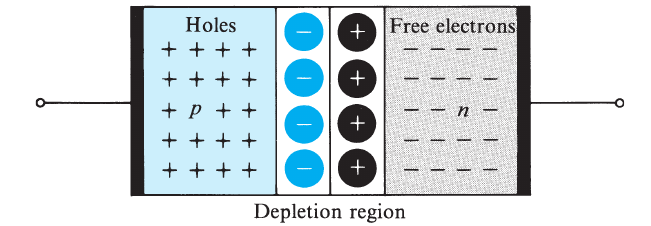
\includegraphics[scale=0.5]{./Depletion_Layer.png}
  \caption{Depletion Layer (\cite[p.~150]{sedraTextbook7})}
  \label{fig:Depletion_Layer}
\end{figure}

We can find the width of the \nameref{def:Depletion_Layer} using \Cref{eq:Depletion_Layer_Width}.
\begin{equation}\label{eq:Depletion_Layer_Width}
  \DepletionDistance = \sqrt{\frac{2 \SiElectricPermittivity}{\eCharge} \left( \frac{1}{\AcceptorConcentration} + \frac{1}{\DonorConcentration} \right) \JunctionBuiltInVoltage}
\end{equation}

The depletion layer ``bleeds'' into each side of the \PNJunction{}.
We can find the distance the depletion layer falls into each side with \Cref{eq:Depletion_Layer_Directions-Electron,eq:Depletion_Layer_Directions-Hole}.

\begin{subequations}\label{eq:Depletion_Layer_Directions}
  \begin{equation}\label{eq:Depletion_Layer_Directions-Electron}
    x_{\Electron} = \DepletionDistance \left( \frac{\AcceptorConcentration}{\AcceptorConcentration + \DonorConcentration} \right)
  \end{equation}
  \begin{equation}\label{eq:Depletion_Layer_Directions-Hole}
    x_{\Hole} = \DepletionDistance \left( \frac{\DonorConcentration}{\AcceptorConcentration + \DonorConcentration} \right)
  \end{equation}
\end{subequations}

Lastly, the sum of the ``bleed'' in both directions is equal to the width of the entire \nameref{def:Depletion_Layer}.
\begin{equation}\label{eq:Depletion_Layer-Directions_Sum}
  \DepletionDistance = x_{\Electron} + x_{\Hole}
\end{equation}

%%% Local Variables:
%%% mode: latex
%%% TeX-master: "../ECE_311-Engineering_Electronics-Reference_Sheet"
%%% End:
